\newpage

\section*{ $^{98}$Mo(n,$\gamma$)$^{98}$Mo }

Power Level: 100 kW(th) \\
Time at Power: 3600 s \\
Wait Time: 172800 s \\
Total Activity at Removal: 2.51e+00 $\mu Ci$

\begin{table*}[h]
\centering
\begin{tabular}{ |c|c|c|c|c|c| }
 \hline
 Position & Mass $mg$ & Counting Time $s$ & Counting Activity $\mu Ci$ & Expected Area (Counts) \\
 \hline 
 1 & 1.5469220246238031 & 600 & 3.44e-01 & 2.79e+04\\ 
\hline
 2 & 1.5469220246238031 & 600 & 4.97e-01 & 4.04e+04\\ 
\hline
 3 & 1.5469220246238031 & 600 & 4.65e-01 & 3.77e+04\\ 
\hline
 4 & 1.5469220246238031 & 600 & 2.24e-01 & 1.82e+04\\ 
\hline
\end{tabular}
\end{table*}

\begin{figure}[!ht]
   \centering
   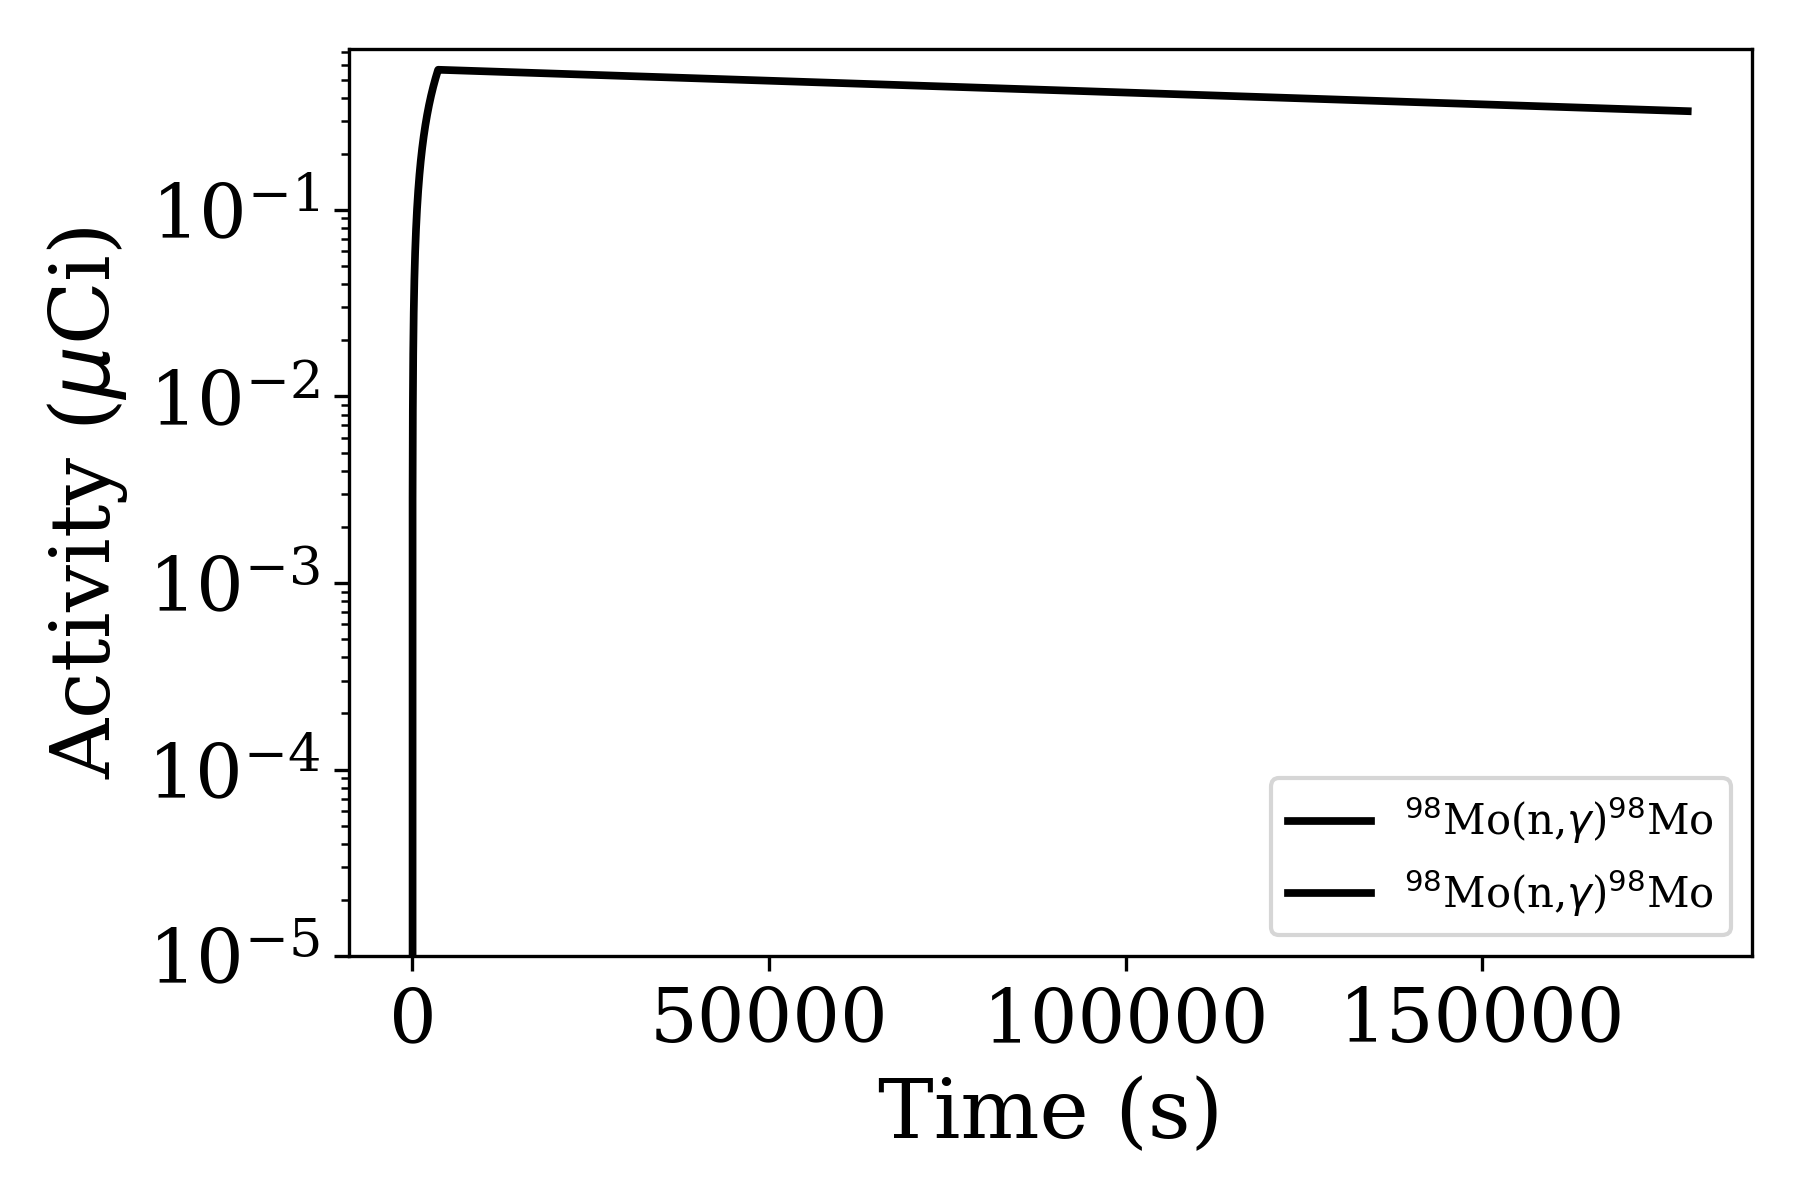
\includegraphics[width=.4\textwidth]{source/plot/Mo-98(n,gamma)Mo-98_wisconsin1.png} 

\end{figure}

\begin{figure}[!ht]
   \centering
   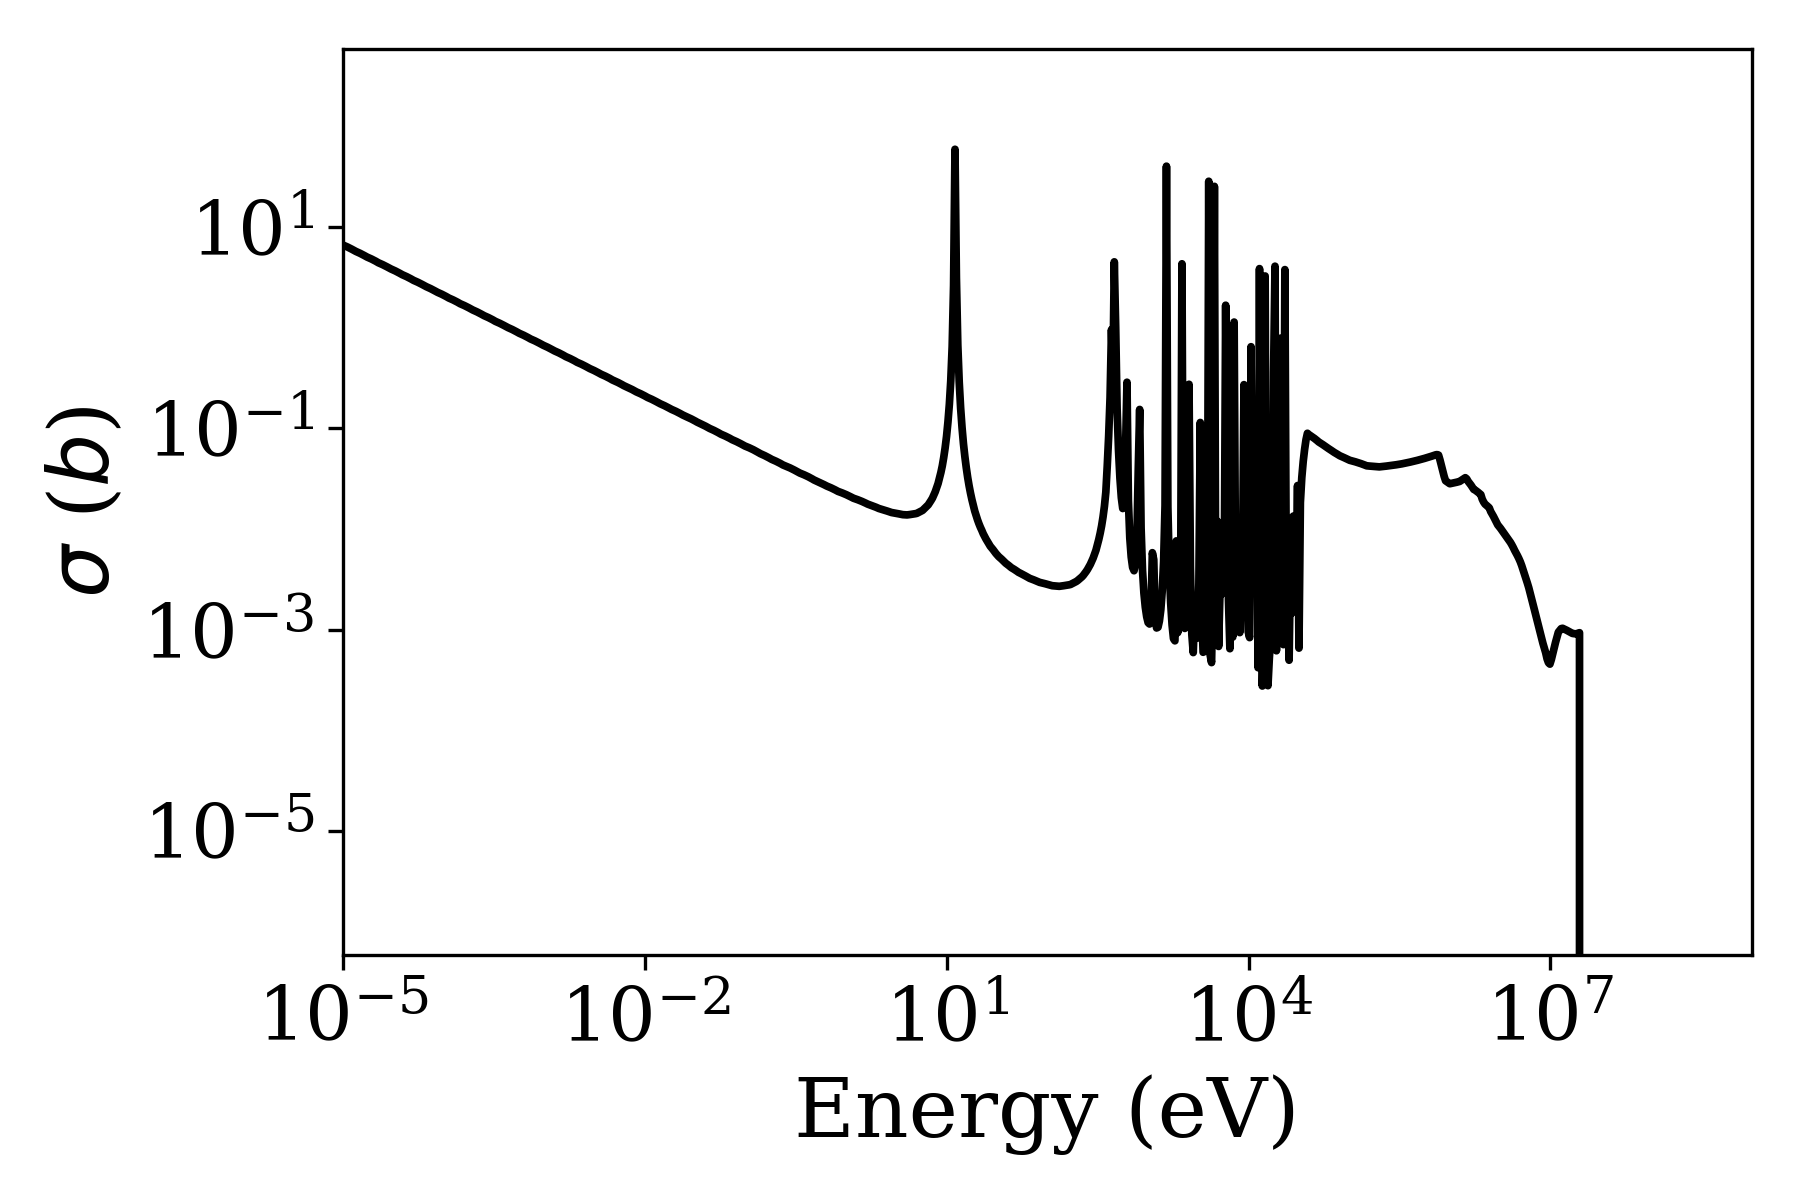
\includegraphics[width=.4\textwidth]{source/plot/Mo-98(n,gamma)Mo-98.png} 

\end{figure}

\begin{table*}[h]
\centering
\begin{tabular}{ |c|c|c|c|c|c|c| }
 \hline
 Reaction & T$_{1/2}$ & ROI (eV) & Important Gammas (keV) \\
 \hline 
 $^{98}$Mo(n,$\gamma$)$^{98}$Mo &  2.8 d & 2.96e-02, 2.26e+05 & 740(0.12),  \\ 
\hline
\end{tabular}
\end{table*}
